% ============================================================================
% sec1_intro.tex — Introduction (Plan B version, 2026-11-06)
% Fig.1 = 0.58 width figure*; contributions C1-C4 per Lead execution order.
% ============================================================================
\section{Introduction}
\label{sec:intro}

\begin{figure*}[t]
\centering
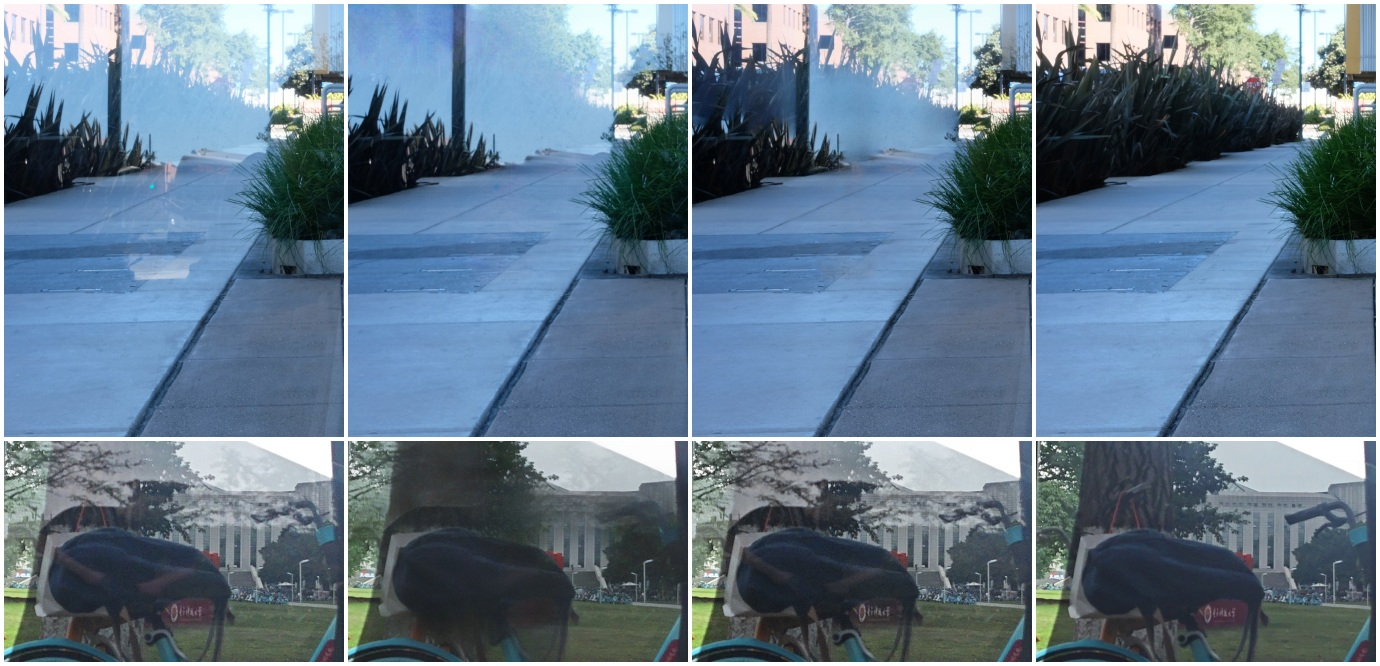
\includegraphics[width=0.58\textwidth]{fig/teaser_2rows.jpg}
\caption{\textbf{Same model, two kinds of glass.} Top: on Real20 a state-of-the-art
method removes the reflection almost completely while a light-weight model removes only
part of it. Bottom: on a filmed-glass pair the same method darkens the frame and strips
transmitted detail instead of removing the reflection, and the light-weight model
changes almost nothing. The difference is not the network but the imaging: the film sits
on the scene side, so transmitted light is scattered and dyed while the reflection comes
off the bare glass surface.}
\label{fig:teaser}
\end{figure*}

Single-image reflection removal (SIRR) addresses a situation any camera user has met:
a photograph through a pane of glass, in which the scene behind the camera is
superimposed on the scene in front of it. The setting---car windows, shop facades,
museum cases, aquaria---is ubiquitous; SIRR is a standing task.
The dominant recipe is data-driven: paired corpora, a network
regressing the transmitted layer, and a loss on deviation from the clean
reference. Successive generations---classical layer priors, cascaded and recurrent
designs, reversible and dual-stream architectures, and recently diffusion
priors~\cite{wan2017benchmarking,wan2022crrn,li2020ibcln,wen2019errnet,zhao2025rdnet,hu2024dsit,hu2023dsrnet,hong2024ldiffer,promptrr2024,li2026gensirr,hu2026dai,xu2026fumo}---have
advanced the state of the art on benchmarks such as
Real20~\cite{zhang2018perceptual} and SIR$^2$~\cite{wan2017benchmarking}.

What these recipes share is an assumption about the \emph{glass}. In deployment the
glass is rarely bare: automotive and architectural glazing is almost always
\emph{filmed}, for heat rejection, privacy and UV protection, and a dark film changes
the imaging. The film is laminated on the scene side, so the light we want travels
through it---scattered, absorbed and dyed---while the light to discard comes off the bare
surface facing the camera. The observed image is a sharp
reflection over a soft, desaturated transmission: the layers separate in band and
chroma, not in level. Methods trained on ordinary glass do not expect this, and
empirically do not survive it (Fig.~\ref{fig:teaser}).

SIRR has been attacked with stronger backbones, reversible connections, reflection-rate
estimates and generative priors. What these efforts
share is where they are measured: on benchmarks whose reflections are dense and cover
most of the frame, so a whole-image average already describes the failure. Three things
are consequently missing: to our knowledge, no real paired dataset shot through filmed
glass has been released, so the regime cannot be measured; no analysis of \emph{where}
a method fails, because one average cannot separate regions where removal is necessary
from those where it is harmful; and, consequently, training losses inherited from
dense-reflection settings.

This paper takes the opposite order. We first ask what filmed glass does to the two
layers and measure: the transmitted layer loses high-frequency content while the
reflection stays sharp, so detail and discardable content separate in band rather than
brightness (Sec.~\ref{sec:imaging}). We then
ask \emph{where} current methods fail: the reflection is weakest inside the region
blocked by the photographer, where almost nothing needs to change, and strongest in the
annulus around it, which is large and where each of the baselines we tested is at its
worst; because it borders a nearly correct region, its residual is read by the eye as a
\emph{boundary} (Sec.~\ref{sec:diagnosis}). Finally we ask what training signal
achieves. A region-relative error is the load-bearing term in development ablations; an
area-matched random-region control indicates that its value comes from normalising by the
local reflection amplitude rather than from the region's identity, so we reduce it to a
mask-free per-pixel regularizer (Sec.~\ref{sec:method}) and test it as a controlled
intervention against identity, magnitude-matched, hard-threshold and shuffled controls
under one training recipe (Sec.~\ref{sec:exp}). We close by stating what the development
panel can and cannot support (Sec.~\ref{sec:discussion}).

\paragraph{Contributions.}
\begin{itemize}
\item \textbf{Data.} A hand-annotated 15-scene real-pair development benchmark for filmed
glass, with training pairs from sessions with locked exposure and white balance and an
explicit quantification of the capture defects (Secs.~\ref{sec:imaging}--\ref{sec:panel}).
\item \textbf{Diagnosis.} A diagnosis organized around two failure axes---transmission
loses high-frequency content while reflection stays sharp (an empirical layer
asymmetry), and the global photometric level is not identifiable from a single
frame---with current methods failing in the annulus around the occluder region
structurally rather than photometrically (Sec.~\ref{sec:diagnosis}).
\item \textbf{Protocol.} A pre-registered, unified-recipe control protocol: a mask-free
change-aware regularizer tested against identity, magnitude-matched, hard-threshold and
shuffled controls over three seeds, bounding what training-time regularization achieves
on this benchmark while disclosing run-level reproducibility (Sec.~\ref{sec:exp}).
\item \textbf{Boundary.} An honest statement of where claims stop: occluder-region
specificity is withdrawn, no public-benchmark state-of-the-art claim is made, the panel
is a development panel with a stated minimum detectable effect, and several negative
results are reported (Sec.~\ref{sec:discussion}).
\end{itemize}

\paragraph{Organisation.} Sec.~\ref{sec:related} reviews related work;
Secs.~\ref{sec:imaging}--\ref{sec:method} present the study;
Secs.~\ref{sec:exp}--\ref{sec:discussion} report experiments and limitations.
